\section{RQ3: Can the Full Suite Detect Slowdowns in Code It Reaches?}
\label{sec:rq3}

\paragraph*{Detection of the frozen slowdowns}
Fig.~\ref{fig:slowdowns} decomposes the \NumSlowdowns{} frozen slowdowns on networkx.
The full suite flags \SlowDetClassified{} of them (Wilson \ci{\SlowDetClassLo}{\SlowDetClassHi}) and \SlowDetOnTarget{} on target (\ci{\SlowDetOnTargetLo}{\SlowDetOnTargetHi}), where ``on target'' means the flagged case executes the slowed function in its profile.
Slowdown \#2 (\texttt{\_dijkstra\_multisource}) is detected by all \SlowTwoCases{} profiled cases at \SlowTwoRatioLo--\SlowTwoRatioHi\x{}, and \#8 (\texttt{\_build\_paths\_from\_predecessors}, list membership) by its one profiled case at \SlowEightRatio\x.
The third flag, \#1, is off target: its only slower case (\SlowOneRatio\x, exact $p=\SlowOneExactP$) never executes \texttt{bidirectional\_dijkstra}, and the patch changes only that function's body.
One rule decides all flags: a flag counts as a detection only if the flagged case executes the slowed function in its profile; flags on cases that do not are reported as off target and are not counted, whatever their size.
By that rule \#1 is not a detection.
Across the oracle there were \OffTargetVerdictable{} off-target comparisons that can yield a verdict (plus fifty spot-check comparisons that cannot, \OffTargetComparisons{} in all); at $\alpha=\AsvAlpha$ about \OffTargetExpected{} false non-``same'' verdicts are expected, and \OffTargetObserved{} were observed (Poisson upper tail $\approx\OffTargetPTail$), consistent with chance.
The two on-target detections are not equally strong: \#2 rests on all its profiled cases at ratios far above the threshold, while \#8 rests on one case just above the ratio condition, inside the noise band of comparable A/A cases.
\TODO{E2/E3: state for \#2 and \#8 whether they pass the $1+3\sigma$ floor and reproduce on repetition; if \#8 does not, the on-target count becomes one.}

\begin{figure}[t]
\centering
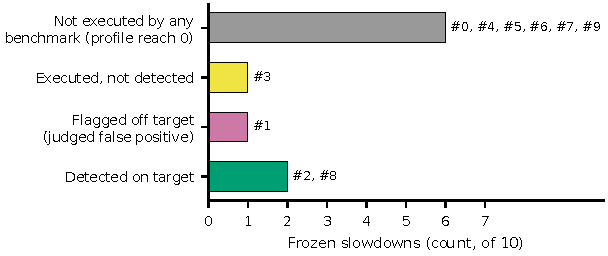
\includegraphics[width=\columnwidth]{figures/fig_slowdowns.pdf}
\caption{The frozen slowdowns on networkx by outcome under the full suite: not executed by any benchmark (coverage miss), executed but not detected, detected on target, and flagged off target.}
\label{fig:slowdowns}
\end{figure}

\paragraph*{Three factors: executed, visible, detectable}
Whether the oracle can see a slowdown in a function depends on three factors in turn: some benchmark must \emph{execute} the function (coverage, RQ2); the function must take a large enough \emph{share} of that benchmark's time for the slowdown to be visible at the case level; and the case-level effect must be \emph{detectable} above the noise (power).
We estimated the share for each profile-reaching case with cProfile at the slowdown's state (unpatched), as the slowed function's inclusive time over the case's profiled time; cProfile overhead inflates call-heavy code, so the shares are approximate.
For a slowdown that calls the function body twice, the expected case-level ratio is about one plus the share.

\textbf{Coverage misses.} Of the \SlowMissed{} slowdowns the full suite misses, \SlowMissedUnreached{} are in functions that no benchmark reaches by profile or by static reach.
\#4 (\texttt{\_single\_shortest\_path}) is executed by no case in its measured profile, so it is a coverage miss as well.
Static reach does not separate these slowdowns: the $S_0$ static call graph connects all \NxBenchCases{} cases to each of \#1--\#4 and \#8, because the heavy benchmark module imports most of the package.
At this granularity static reach is uninformative, so we classify reach by the measured profile only: no case for \#1 and \#4, three for \#3, \SlowTwoCases{} for \#2 and one for \#8.
In total, \SlowUnreachedProfile{} of the \NumSlowdowns{} slowed functions are executed by no benchmark case in its profile, consistent with RQ2.

\textbf{A share miss.} \#3 (\texttt{is\_connected}) is executed by three profiled cases of the heavy module, but takes only \ShareThreeLo--\ShareThreeHi{} of their time, so doubling it should change them by a ratio of about \ExpThree, far below asv's factor of \AsvFactor{} and any noise floor; the observed ratios stayed near one.
\#3 is therefore a miss of a diluted effect, not a lack of power: no number of repetitions would make it visible to these cases.

\textbf{Detections match the share.} For \#2 the share is \ShareTwoLo--\ShareTwoHi, which predicts ratios close to the observed \SlowTwoRatioLo--\SlowTwoRatioHi.
For \#8 the share is \ShareEight, but its slowdown changes one membership test inside the function rather than doubling the body, so one plus the share does not predict its ratio.

No selection rule can detect more than the full suite, so on networkx coverage, share and power limit regression detection before any selection does.
As a consequence, the pre-registered primary result on regression safety of reduced benchmark selection is that it is \emph{not measurable} with this frozen set: no slowdown was detected on target within the pre-registered strength bands.

\paragraph*{Noise floor}
In the A/A control, asv's rule gave \AAFalse{} false verdicts in \AAComparisons{} per-repeat comparisons (Wilson upper bound \AAUpper\pct).
The \AAComparisons{} comparisons are the same \AACases{} cases twice, so the bound is optimistic.
The noise sits near the threshold: some cases passed the $p$ condition and stayed ``same'' only on the ratio condition, and under a fixed run order one case reached a ratio of \AAMaxSameRatio{} without passing the $p$ condition.
\TODO{E2 ($\sigma$ for flagged cases, overnight 22--23 Nov): $\sigma$ from five A/A repeats (ABBA) for every case with a slower verdict (\#1, \#2's cases, \#8, \#9) and a seeded sample of the heavy-module cases; apply the pre-registered $1+3\sigma$ floor to every verdict and report which survive. Until then no verdict in this section has passed the floor.}

\paragraph*{Power}
A bootstrap from the A/A samples under the exact test (Fig.~\ref{fig:power}) gives a median detection probability of \PowAllOneTwo{} at a slowdown of \PowFactorMid\x{} over all A/A cases, but only \PowAlgoOneTwo{} for the \AAAlgoCases{} sampled cases of the heavy module; at \PowFactorHigh\x{} the values are \PowAllTwo{} and \PowAlgoTwo.
The bootstrap ignores the correlation of samples within a process, so these values are optimistic.
In the module that holds most of the cost, then, the bootstrap reaches high detection probability only for large slowdowns; the \AAAlgoCases{} sampled cases are a small part of that module, no factor between the two was bootstrapped for this figure's headline, and the estimate is optimistic, so this is indicative only.
\TODO{E2: enlarge the heavy-module A/A sample (at least ten seeded cases), report the power at each bootstrapped factor with an interval, and replace ``large slowdowns'' with the measured factor.}
\TODO{Fig.~\ref{fig:power}: add the measured graded slowdowns (1.1, 1.2, 1.5, 2$\times$ in 3--4 reached functions) as points, if run; otherwise state that the curve is a bootstrap estimate only.}

\begin{figure}[t]
\centering
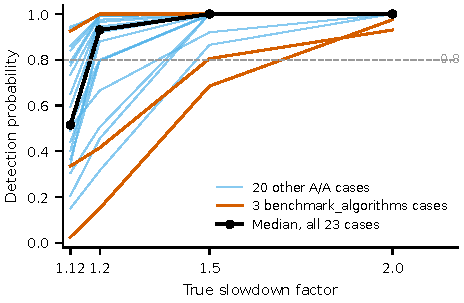
\includegraphics[width=\columnwidth]{figures/fig_power.pdf}
\caption{Bootstrap detection probability of asv's rule under the exact Mann-Whitney test, by slowdown factor, for the A/A cases on networkx. The heavy-module curve rests on three sampled cases.}
\label{fig:power}
\end{figure}

\paragraph*{Repeatability}
\TODO{E3 (repeated slowdown oracle, tonight): re-run the oracle for the slowdowns with at least one case in profile or static reach (\#1, \#2, \#3, \#4, \#8) with ABBA, five processes and at least two repeats; report verdict agreement and whether \#1 reproduces (noise or not).}

\paragraph*{Statistics}
The rule we first implemented used scipy's default Mann-Whitney method, a normal approximation at these sample sizes, while asv uses an exact test.
Re-testing all \RecomputeVerdicts{} verdicts from their raw samples under the exact test changed \RecomputeChanged{} of them; borderline $p$ values became smaller.
All $p$ values above are exact.
The smallest attainable two-sided exact $p$ for six against six samples is \MinPSixSix, above $\alpha=\AsvAlpha$, so a spot check of that size can never return ``slower'' (Section~\ref{sec:lessons}); for fifteen against fifteen it is \MinPFifteen.

\paragraph*{Profile completeness}
Benchmarks outside the measured reach of a slowed function should not slow down.
A powered check of the \SlowMissedUnreached{} unreached slowdowns against a seeded sample of out-of-reach cases found \CompletenessSlower{} slower verdict in \CompletenessN{} comparisons: \#9 on a \texttt{louvain\_communities} case at \SlowNineRatio\x{} (exact $p=\SlowNineExactP$).
By the pre-registered rule this flags reach-based selection as unsafe for \#9, and the flag stands as the primary result.
A post-hoc re-check with a second unpatched control did not reproduce it (\SlowNineRecheckLo--\SlowNineRecheckHi\x), which is consistent with one false positive in \CompletenessN{} comparisons but does not prove it.
This is a check of the profiles, not evidence that selection is safe.

\paragraph*{Answer to RQ3}
On networkx, where some benchmark executes a slowed function in its measured profile, the full suite detected the largest injected slowdown (\SlowTwoRatioLo--\SlowTwoRatioHi\x) on every profiled case and a smaller one (\SlowEightRatio\x) once; the noise floor of the heavy module means moderate slowdowns there are likely to go unseen.
Together with RQ2, the oracle's misses split into coverage misses (\SlowUnreachedProfile{} of the \NumSlowdowns{} slowed functions are executed by no benchmark) and a share miss (\#3, executed but too small a part of its benchmarks to be visible), while \#1's only flag is an off-target noise verdict; no miss in this set is attributable to power alone, though the A/A bootstrap says power would limit moderate slowdowns in the heavy module.
